\chapter{Estruturas de dados probabilísticas}\label{cap:probds}

Estruturas de dados probabilísticas permitem estimar propriedades sobre fluxos de dados utilizando menos recursos que suas alternativas determinísticas. Isso é possível através da sub-representação dos dados subjacentes, para compor as operações sobre a estrutura.

Neste capítulo analisaremos quatro estruturas de dados probabilísticas que utilizam funções \emph{hash} para representar operações em conjuntos e multiconjuntos utilizando consideravelmente menos memória que suas representações determinísticas. A Figura~\ref{fig:probds_table} sumariza estas estruturas e as operações que cada uma é capaz de efetuar. Considere $n$ a cardinalidade de elementos distintos destes (multi)conjuntos. Os detalhes de funcionamento de cada uma destas estruturas serão abordados nas próximas seções.
\begin{figure}[!htbp]
\centering
\begin{tabular}{ | c | c | }
\hline
    \textbf{Estrutura} & \textbf{Consulta} \\
\hline
\hline
    \multirow{2}{*}{Filtro de Bloom} &     
    Pertinência \\
\cline{2-2}
    & Cardinalidade \\
\hline
\hline
    \multirow{3}{*}{Count-Min sketch} &      
    Frequência \\
\cline{2-2}
    & Produto escalar \\
\cline{2-2}
    & Somatório de intervalos \\
\hline
\hline
  MinHash & 
  Similaridade \\
\hline
\hline
  HyperLogLog & 
  Cardinalidade \\
\hline
\end{tabular}
\caption{Sumário de estruturas abordadas neste capítulo}
\label{fig:probds_table}
\end{figure}

%~~~~~~~~~~~~~~~~~~~~~~~~~~~~~~~~~~~~
% INCLUDES
%~~~~~~~~~~~~~~~~~~~~~~~~~~~~~~~~~~~~

%~~~~~~~~~~~~~~~~~~~~~~~~~~~~~~~~~~~~~~~~~~~~~~~~~~~~~~~~~~~~~~~~~~~~~~~
\section{Filtro de Bloom}\label{sec:bloom}
%~~~~~~~~~~~~~~~~~~~~~~~~~~~~~~~~~~~~~~~~~~~~~~~~~~~~~~~~~~~~~~~~~~~~~~~

Um filtro de Bloom é uma estrutura de dados probabilística que representa um conjunto e permite verificar a pertinência de elementos com tolerância a falsos positivos \cite{bloom1970space}. É uma representação bastante compacta: são necessários menos de 10 bits por elemento para uma probabilidade 1\% de falsos positivos \cite{bonomi2006improved}. 

\subsection{Definição}\label{sec:bloom:def}

Um filtro de Bloom representa um conjunto $S$ de cardinalidade $n$ utilizando um vetor $B$ de $m$ bits. Inicialmente, $B[i] = 0$ para todo $i \in [1..m]$. O filtro está associado a $k$ funções \emph{hash} $h_i : S \rightarrow [1..m]$, para todo $i \in [1..k]$. Assume-se que cada função $h_i$ mapeia elementos de $S$ naqueles de $[1..m]$ de forma aleatória com uma distribuição uniforme.

Para inserir um elemento, é preciso atribuir 1 para cada posição no filtro mapeada pelas funções $h_i$, como mostra o Algoritmo~\ref{alg:bloominsert}.

\begin{algorithm}
\linespread{1}\selectfont
\caption{Adiciona um elemento a um filtro de Bloom}
\label{alg:bloominsert}
\begin{algorithmic}[1]
\Procedure{Inserir}{$x$}
    \For{$i \gets  1 \textrm{ to } k$}
        \State $B[h_i(x)] \gets 1$
	\EndFor
\EndProcedure
\end{algorithmic}
\end{algorithm}

Analogamente, para verificar se um elemento pertence a um conjunto, é preciso verificar se todos os bits mapeados pelas funções $h_i$ estão ``ligados'', i.e., um elemento $x$ provavelmente pertence ao conjunto $S$ se o Algoritmo~\ref{alg:bloomquery} retorna verdadeiro.

\begin{algorithm}
\linespread{1}\selectfont
\caption{Verifica se um elemento pertence a um filtro de Bloom}
\label{alg:bloomquery}
\begin{algorithmic}[1]
\Function{Verificar}{$x$}
    \State $resultado \gets \textbf{true}$ 
    \For{$i \gets  1 \textrm{ to } k$}
        \State $resultado \gets resultado \land B[h_i(x)] = 1$
	\EndFor
	\Return $resultado$
\EndFunction
\end{algorithmic}
\end{algorithm}

A Figura~\ref{fig:bloom1} mostra um exemplo de filtro de Bloom. Do lado esquerdo, estão representadas as operações de inserção, utilizando duas funções \emph{hash}. Do lado direito, as operações de verificação. Importante notar que na última operação de verificação trata-se de um caso de falso positivo, pois o elemento não existe de fato no conjunto previamente inserido.

\begin{figure}[!htbp]
  \centering
  \includegraphics[scale=0.45]{figures/bloom1.pdf}
  \caption{Exemplo de filtro de bloom}
  \label{fig:bloom1}
\end{figure}

Quando $k=1$, o funcionamento de um filtro de Bloom é similar ao de uma \emph{hash table} tradicional, porém os elementos originais não são armazenados. Em vez disso, apenas um bit é usado para representar a pertinência do \emph{hash} do elemento na tabela. Na prática, múltiplas funções \emph{hash} são utilizadas.

Assim como em tabelas \emph{hash}, pode haver colisões nos filtros de Bloom. Portanto, falsos positivos são possíveis. Falsos negativos por sua vez não são possíveis. Este comportamento é desejado em sistemas que precisam evitar operações custosas (por exemplo, acesso a disco, comunicação de rede, etc.) em casos onde não seja realmente necessário. 

Para diminuir a probabilidade de colisão, é preciso dimensionar o filtro e as funções \emph{hash} baseados no número de elementos esperados. Por exemplo, usando 7 funções e pouco menos de 10 bits por elemento no filtro, é possível garantir uma probabilidade de falsos positivos menor que 1\% \cite{bonomi2006improved}. É possível determinar a quantidade ótima de bits e funções dada uma probabilidade esperada de falsos positivos.

As funções \emph{hash} usadas no filtro precisam ser independentes duas-a-duas, o que pode exigir muitos recursos computacionais. Em \cite{kirsch2006less}, Kirsch e Mitzenmacher mostram que é possível implementar um filtro de Bloom com qualquer valor de $k$ apenas combinando duas funções \emph{hash} independentes, sem aumentar a probabilidade de falsos positivos.

Em termos de operações suportadas, filtros de Bloom permitem atualização incremental, bem como união entre filtros (que para filtros de mesmo número de bits, consiste em uma operação \emph{OU} bit-a-bit entre eles). Entretanto, em sua forma mais simples, não suportam remoção de elementos nem interseção entre filtros sem introduzir falsos negativos ou afetar as probabilidades de falsos positivos. Diversas variações e extensões aos filtros de Bloom foram propostas, algumas discutidas nas Seções \ref{sec:bloom:counting} e \ref{sec:bloom:variants}.

\subsection{Exemplo}\label{sec:bloom:example}

Com o objetivo de facilitar o entendimento da estrutura filtro de Bloom, apresentamos aqui um exemplo prático de seu uso. Consideraremos aqui a simulação de inserção de strings em um filtro de Bloom com $m = 16$, usando duas funções \emph{hash} que retornam valores no intervalo $[0;15]$. A Figura~\ref{fig:bloom_example_legend} explica como será representada cada entrada no exemplo.

\begin{figure}[!htbp]
  \centering
  \includegraphics[scale=0.6]{figures/bloom_example_legend.pdf}
  \caption{Modelo de linha para exemplos}
  \label{fig:bloom_example_legend}
\end{figure}

A simulação é dividida em duas partes: inserções e consultas. Na parte das inserções, cada linha (exceto a primeira) contém uma string a ser inserida e os valores retornados por cada função \emph{hash}. Esses valores representam os índices que serão escritos no vetor. Além disso, para cada string, são representadas as 16 posições do vetor $M$ com o estado após a inserção, destacando os índices referenciados. A primeira linha representa o estado inicial. Na parte das consultas, algumas consultas são representadas da mesma maneira que as inserções, entretanto, o vetor não é modificado. A simulação pode ser vista na Figura~\ref{fig:bloom_example}.

\begin{figure}[!htbp]
  \centering
  \includegraphics[scale=0.6]{figures/bloom_example.pdf}
  \caption{Exemplos de inserção e consultas no filtro de Bloom}
  \label{fig:bloom_example}
\end{figure}

As consultas efetuadas representam resultados diferentes. A consulta por \texttt{Ford Prefect} retorna um resultado positivo, pois ambos os índices apontam para valores 1 na tabela, indicando que a string de fato existe no conjunto. A consulta por \texttt{Slartibartfast} retorna um resultado negativo, pois um dos índices aponta para um valor 0 na tabela, indicando que a string não existe no conjunto. Este resultado é dado com 100\% de certeza. A consulta por \texttt{Fenchurch} retorna um resultado positivo, porém este é um falso positivo, visto que esta string não faz parte do conjunto.

\subsection{Probabilidade de falso positivo}\label{sec:bloom:false}

A probabilidade de um falso positivo é determinada pela probabilidade de colisão. Assim, quanto mais bits forem usados no filtro de Bloom, menor a probabilidade de um falso positivo. Para diminuir a probabilidade de colisões é possível também utilizar múltiplas funções \emph{hash} para cada elemento, mas somente até um certo ponto, onde realizar múltiplos hashes por elemento acaba aumentando a probabilidade de colisões.

É possível calcular a probabilidade de um falso positivo. Considere uma tabela $B[1..m]$, após inserir os elementos do conjunto $X$, com $|X| = n$, e usando $k$ funções \emph{hash}. Se $X_i$ é a variável aleatória que fornece o valor de $B[i]$, então:
\[
\Pr[X_i = 0] = \Pr\left[\bigwedge_{x \in X, 1 \leq j \leq k} h_j(x) \neq i \right] = \left( 1 - \frac{1}{m}\right)^{kn}
\]

Seja \textsc{FalsoPositivo} o evento do filtro reportar pertinência para um elemento $x \notin X$. Logo, a probabilidade de haver um falso positivo é a mesma de encontrar $k$ bits 1 aleatoriamente na tabela, ou seja:
\[
\Pr[\textsc{FalsoPositivo}] = \Pr\left[\bigwedge_{1 \leq j \leq k} X_{h_j(x)} = 1 \right] = \left( 1 - \left( 1 - \frac{1}{m}\right)^{kn} \right)^k \approx \left( 1 - \mathrm{e} ^{-kn/m} \right)^k
\]

A aproximação acima se dá pois $(1 - x)^y \approx \mathrm{e}^{-xy}$, conforme $x$ se aproxima de zero. É fácil ver que a probabilidade de falsos positivos cresce conforme $n$ cresce. Por isso, é preciso dimensionar o filtro de Bloom de acordo com o número de elementos no conjunto. Se definirmos $q = m/n$ (quantidade de bits por elemento, reescrevemos a última probabilidade como:
\[
\Pr[\textsc{FalsoPositivo}] \approx \left( 1 - \mathrm{e} ^{-k/q} \right)^k
\]

A Figura~\ref{fig:probfalso1} mostra como esta probabilidade se comporta para diferentes valores de $k$ e $q$. Bonomi et al. \cite{bonomi2006improved} mostram ainda que a probabilidade é minimizada quando $k = q \ln 2$. Assim, é possível definir a probabilidade mínima de falsos positivos a partir do número de bits por elemento:
\[
\Pr[\textsc{FalsoPositivo}] = (1-e^{\ln(2)}) ^ {q \ln(2)} = ((1/2)^{\ln(2)})^q \approx \left( 0,6185 \right)^q
\]

\begin{figure}[!htbp]
\centering
\scalebox{0.80}{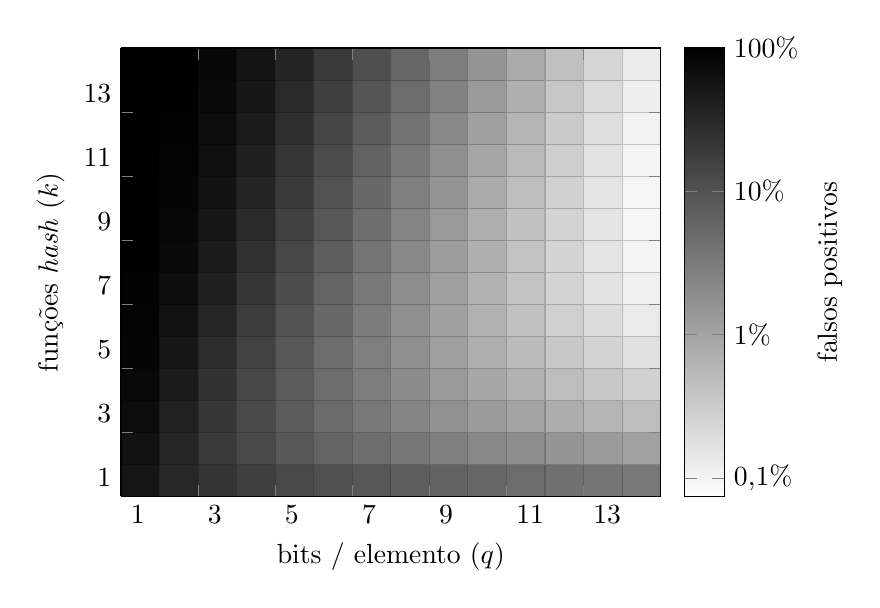
\begin{tikzpicture}[
        declare function = {
            p(\q,\k) = ((1 - (e^(-\k/\q)))^\k)*100;
        }
    ]
    \begin{axis}[
        view={0}{90}, 
        colorbar, 
        colorbar style={
            ylabel=falsos positivos,
            yticklabels={0, {0,1\%}, 1\%, 10\%, 100\%},
        },
        colormap={}{ gray(0cm)=(1); gray(1cm)=(0);},
        xlabel=bits / elemento ($q$),
        ylabel=funções \emph{hash} ($k$),
        xticklabel style={anchor=north west},
        yticklabel style={anchor=south east},
        ytick = { 1, 3, ..., 14},
        xtick = { 1, 3, ..., 14},
        zmode=log,
        log base z=10,
    ]
        \addplot3[surf,domain=1:15,samples=15]{p(x,y)};
    \end{axis}
\end{tikzpicture}}
\caption{Probabilidade de falsos positivos}
\label{fig:probfalso1}
\end{figure}

É possível ver na Figura~\ref{fig:probfalso2} que a probabilidade de falsos positivos cai exponencialmente em relação ao número de bits por elemento no filtro.

\begin{figure}[!htbp]
\centering
\scalebox{0.80}{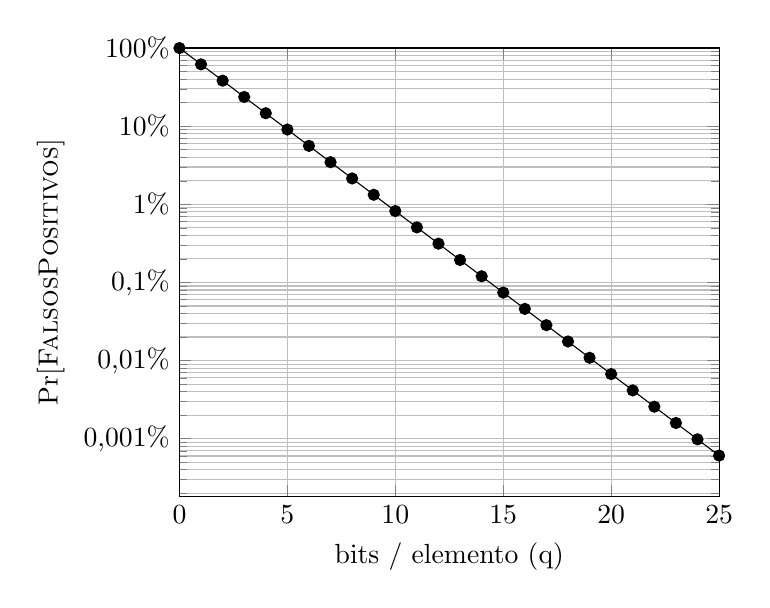
\begin{tikzpicture}[
        declare function = {
            p(\q) = (0.6185)^(\q);
        }
    ]
	\begin{axis}[
        grid=both,
        xlabel=bits / elemento (q),
		ylabel={Pr[\textsc{FalsosPositivos}]},
        yticklabels={0, {0,001\%}, {0,01\%}, {0,1\%}, 1\%, 10\%, 100\%},
        ymode=log,
        ymax=1,
		xmin=0,
		xmax=25]
	\addplot[mark=*,domain=0:25,samples=26] {p(x)};
	\end{axis}
\end{tikzpicture}}
\caption{Probabilidade mínima de falsos positivos}
\label{fig:probfalso2}
\end{figure}

Desta forma, a escolha do número de bits por elemento torna-se crucial para dimensionar a quantidade de falsos positivos. Esta análise precisa ser feita \emph{a priori}, pois não é possível redimensionar um filtro de Bloom sem modificar suas propriedades estatísticas. 

Existem variações do algoritmo que mitigam este problema. Por exemplo, os \emph{Dynamic Bloom Filters} \cite{guo2010dynamic} colocam um limite superior na probabilidade de falso positivo criando um novo filtro quando o limite é ultrapassado, penalizando as consultas em um fator logaritmico, em relação ao tamanho do conjunto, pois precisam verificar vários filtros. Já os \emph{Block-partitioned Bloom Filters} \cite{papapetrou2010cardinality} penalizam tanto a inserção quanto a consulta de forma similar, porém por inserir e verificar os elementos em todos os filtros, mantêm as propriedades algébricas de união entre filtros através de operações booleanas entre seus vetores.

\subsection{Estimativa de cardinalidade}\label{sec:bloom:cardinality}

É possível estimar a cardinalidade do conjunto representado por um filtro de Bloom \cite{whang1990linear,papapetrou2010cardinality}. O princípio é análogo àquele empregado na seção anterior para estimar a probabilidade de falsos positivos. Seja $T$ a variável aleatória que representa o número de bits $1$ após inserir $n$ elementos num filtro $B[1..m]$ e $k$ funções \emph{hash}. Portanto, $T = \sum_{1 \leq i \leq m} X_i = 1$ e a esperança $E[T]$ é uma função $S(n)$ (para $m$ e $k$ fixos) tal que:
\[
S(n) = E[T] = \sum_{1 \leq i \leq m} E[X_i] = m \times Pr[X_i = 1] = m \times \left( 1 - \left( 1 - \frac{1}{m}\right)^{kn} \right)
\]

Desta forma, é possível estimar $n$ a partir do número $t$ de bits 1 existentes no filtro:
\[
n = \hat{S}^{-1}(t) = \frac{\ln \left( 1 - \frac{t}{m} \right)}{k \times \ln \left( 1 - \frac{1}{m} \right)} \approx \frac{-m}{k} \times \ln \left( 1-\frac{t}{m} \right)
\]

A aproximação acima se dá pois $\ln(1 + x) \approx x$, conforme $x$ se aproxima de zero. Perceba que esta estimativa é extremamente dependente da quantidade de bits por elemento no filtro. Portanto, dado um certo filtro de Bloom, apenas um intervalo definido de cardinalidades tem um erro dentro de um limite aceitável. Papapetrou et al. \cite{papapetrou2010cardinality} mostram que é possível definir um limite inferior na probabilidade da cardinalidade real estar num certo intervalo $(n_a, n_b)$ (com $S^{-1}(t-1) \leq n_a \leq n_b \leq S^{-1}(t+1)$). Esta probabilidade se dá pela fórmula:
\[
Pr[n_a \leq n \leq n_b] \geq 1 - e^{-\frac{(t+1-S(n_b))^2}{2S(n_b)}} - e^{t-1-S(n_a)} \times \left( S(n_a) / (t-1) \right)^{t-1}
\]

Este é apenas um limite inferior. Na prática é possível estimar valores bem maiores. Em especial, para estimar cardinalidades não há vantagens em utilizar múltiplas funções \emph{hash}, pois isto somente aumentaria a densidade de bits iguais a 1 no filtro. Whang et al. introduziram o algoritmo \textsc{Linear Counting} \cite{whang1990linear} que utiliza um filtro de Bloom com apenas uma função \emph{hash} para estimar a cardinalidade. Assim,
\[
\hat{n} \approx -m \times \ln \left( 1-\frac{t}{m} \right)
\]

Em  \cite{whang1990linear} também é mostrado que o erro padrão da estimativa está fortemente atrelada ao fator de carga, que consiste em quantos elementos distintos foram inseridos para cada bit na estrutura, ou $n/m$, expresso a seguir:
\[
\sigma_{\hat{n}} = \frac{\sqrt{m(e^{n/m} - (n/m) - 1)}}{n}
\]

Assim, assumindo um filtro com quantidades diversas de bits ($m$), é possível ver a degradação do erro padrão conforme o fator de carga aumenta (Figura \ref{fig:bloom_cardinality}).

\begin{figure}[!htbp]
\centering
\scalebox{0.80}{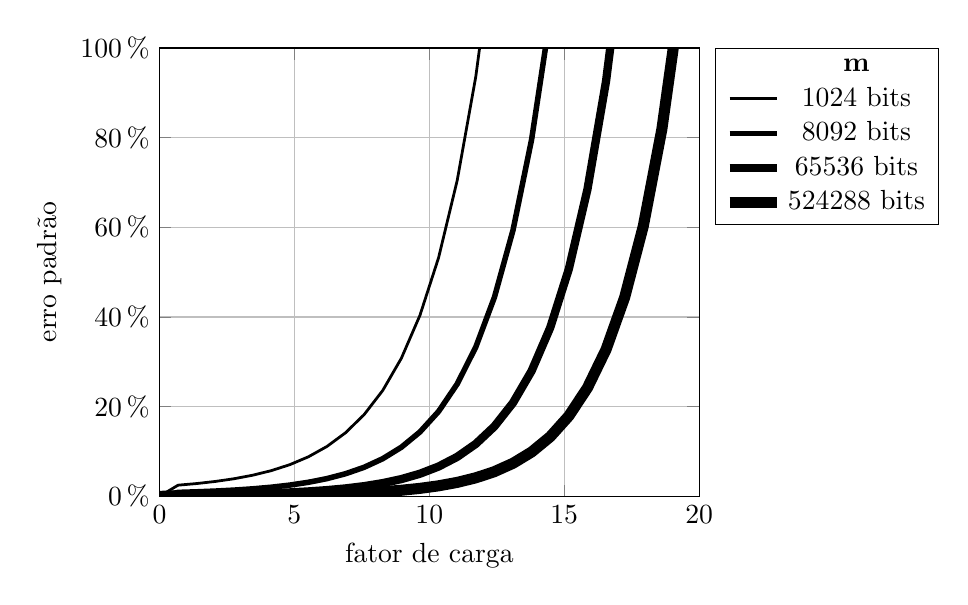
\begin{tikzpicture}[
        declare function = {
            p(\n,\m) = (\m*(e^(\n/\m) - (\n/\m) - 1)) ^ (1/2) / \n;
        }
    ]
	\begin{axis}[
	    scaled ticks=false, 
        grid=both,
        xlabel=fator de carga,
		ylabel=erro padrão,
		yticklabel=\pgfmathparse{100*\tick}\pgfmathprintnumber{\pgfmathresult}\,\%,
		ymin=0, ymax=1,
		xmin=0, xmax=20, 
		legend columns=1, 
	    legend style={legend pos=outer north east,},
    ]
    
    \addlegendimage{empty legend}
            
    \addplot[line width=1pt,domain=0:20,samples=30]{p(1024*x, 1024)};
    \addplot[line width=2pt,domain=0:20,samples=30]{p(8092*x, 8092)};
    \addplot[line width=3pt,domain=0:20,samples=30]{p(65536*x, 65536)};
    \addplot[line width=4pt,domain=0:20,samples=30]{p(524288*x, 524288)};
	\legend{\textbf{m}, 1024 bits, 8092 bits, 65536 bits, 524288 bits};

	\end{axis}
\end{tikzpicture}}
\caption{Erro padrão por fator de carga para filtros de vários tamanhos.}
\label{fig:bloom_cardinality}
\end{figure}

\subsection{\emph{Counting Bloom filters}}\label{sec:bloom:counting}

Em sua forma mais simples, o filtro de Bloom não permite remoção de elementos. Uma solução trivial para este problema, introduzida por Fan et al. \cite{fan1998summary}, é manter um contador de $b$ bits para cada posição no vetor $B$ do filtro.

Desta forma, as operações originais do filtro de Bloom são estendidas. A inserção passa a incrementar o valor de cada uma das posições resultantes das funções \emph{hash} (Algoritmo~\ref{alg:cbloominsert}). A remoção (Algoritmo~\ref{alg:cbloomremove}) e verificação (Algoritmo~\ref{alg:cbloomquery}) são análogas.


\begin{algorithm}[!htbp]
\linespread{1}\selectfont
\caption{Adiciona um elemento a um \emph{Counting Bloom Filter}}
\label{alg:cbloominsert}
\begin{algorithmic}[1]
\Procedure{Inserir}{$x$}
    \For{$i \gets  1 \textrm{ to } k$}
        \If{$B[h_i(x)] < 2^b-1$}
            \State $B[h_i(x)] \gets B[h_i(x)]+1$
        \EndIf
	\EndFor
\EndProcedure
\end{algorithmic}
\end{algorithm}

\begin{algorithm}[!htbp]
\linespread{1}\selectfont
\caption{Remove um elemento de um \emph{Counting Bloom Filter}}
\label{alg:cbloomremove}
\begin{algorithmic}[1]
\Procedure{Remover}{$x$}
    \For{$i \gets  1 \textrm{ to } k$}
        \If{$B[h_i(x)] < 2^b-1$}
            \State $B[h_i(x)] \gets B[h_i(x)]-1$
        \EndIf
	\EndFor
\EndProcedure
\end{algorithmic}
\end{algorithm}    

\begin{algorithm}[!htbp]
\linespread{1}\selectfont
\caption{Verifica se um elemento pertence a um \emph{Counting Bloom Filter}}
\label{alg:cbloomquery}
\begin{algorithmic}[1]
\Function{Verificar}{$x$}
    \State $resultado \gets \textbf{true}$ 
    \For{$i \gets 1 \textrm{ to } k$}
        \State $resultado \gets resultado \land B[h_i(x)] \geq 1$
	\EndFor
	\Return $resultado$
\EndFunction
\end{algorithmic}
\end{algorithm}

Agora a Figura~\ref{fig:bloom2} mostra um exemplo de filtro de Bloom com contagem. Do lado esquerdo figuram as operações de inserção, com duas funções \emph{hash}. Perceba que colisões incrementam a posição resultante no vetor. Do lado direito estão as verificações. Na terceira verificação nota-se um falso positivo.

\begin{figure}[!htbp]
  \centering
  \includegraphics[scale=0.45]{figures/bloom2.pdf}
  \caption{Exemplo de filtro de bloom com contagem}
  \label{fig:bloom2}
\end{figure}

A remoção neste filtro baseia-se na ausência de \emph{overflows} (quando um valor do vetor $B$ atinge $2^b$) em seus contadores. Para tanto, é preciso dimensionar o tamanho destes contadores de forma a minimizar a probabilidade de overflow. Como originalmente o filtro usa apenas um bit por posição no vetor, qualquer número de bits adicionais escolhidos para representar o contador aumenta significativamente o espaço necessário para armazenar a estrutura. Normalmente, 4 bits são suficientes para a maior parte das aplicações, o que faz com que estes filtros usem quatro vezes mais espaço que filtros normais.

O número de bits por contador determina a probabilidade de \emph{overflow}. \emph{Overflows} em \emph{counting Bloom filters} precisam ser tratados. Se um \emph{overflow} ocorrer é preciso manter o contador no máximo valor possível. De forma equivalente, ao tentar decrementar uma posição já no maior valor possível, é preciso mantê-la nesse mesmo valor. Faz-se isto para evitar a introdução de falsos negativos.

Na prática, entretanto, \emph{overflows} devem ser consideravelmente raros. A probabilidade de um \emph{overflow} dado que cada contador usa $b$ bits, após inserir $m$ elementos, usando 10 bits por elemento e otimizando o número de funções \emph{hash} é:
\[
Pr[\textsc{overflow}] \leq n \left( \frac{\mathrm{e} \ln 2}{2^b} \right)^{2^b}
\]
como provado por Fan et al. \cite{fan1998summary}. Assim, ao usar 4 bits para os contadores, a probabilidade de overflow concentra-se em:
\[
Pr[\textsc{overflow em 4 bits}] \leq 1,37 \times 10^{-15} \times n
\]

Esta probabilidade baseia-se na possibilidade de produzir funções \emph{hash} realmente aleatórias, o que pode ser aproximado, mas não pode ser garantido. Em um pior caso em especial, se o mesmo elemento for repetidamente oferecido à estrutura, a probabilidade de \emph{overflow} torna-se criticamente alta.

\subsection{Outras variantes}\label{sec:bloom:variants}

O filtro de Bloom, em sua simplicidade, tem limitações que posam como desafios para algumas aplicações. Desde sua concepção, entretanto, muitas extensões foram propostas para superar estas limitações (geralmente em detrimento de algum parâmetro de desempenho), entre elas:

\begin{description}

  \item[\emph{Compressed Bloom Filters} \cite{mitzenmacher2002compressed}] 
    Discute esquemas de compressão para otimizar o tamanho de filtros enviados através de rede ou salvos em disco. O objetivo é construir filtros com mais bits e menos funções \emph{hash}, de forma a minimizar o tamanho comprimido e/ou aumentar a precisão. Especialmente útil em caso de caches distribuídos. 

  \item[\emph{Distance-sensitive Bloom Filters} \cite{kirsch2006distance}] 
    Responde consultas do tipo ``algum elemento próximo a $x$ pertence a $S$?'', dada uma métrica apropriada, utilizando funções \emph{hash} sensíveis a localidade, com possibilidade tanto de falsos positivos como falsos negativos. Esta variante é bastante útil para detecção de plágio, por exemplo.

  \item[\emph{Dynamic Bloom Filters} \cite{guo2010dynamic}] 
    Permite redimensionar dinamicamente filtros de Bloom sem perder suas propriedades estatísticas. Baseia-se na criação de múltiplos filtros com um limite superior na probabilidade de falsos positivos, i.e., quando um filtro alcança uma taxa de falsos positivos muito alta, outro filtro vazio é criado. Nesta modalidade, a complexidade das operações padrão é maior, entretanto, na prática isso não posa como um problema. É possível dimensionar o tamanho dos filtros a serem criados de forma a amortizar a quantidade de filtros criados ao longo do tempo.

  \item[\emph{Spectral Bloom Filters} \cite{cohen2003spectral}] 
    É uma estrutura especializada em lidar com multiconjuntos. Um \emph{Spectral Bloom Filter} (SBF) funciona praticamente da mesma forma que um \emph{Counting Bloom Filter}, mas suas operações são especializadas em obter a cardinalidade de um certo item num multiconjunto. Nesta estrutura, a cardinalidade de um elemento $x$ se dá por $\displaystyle \min_{i = 1 \dots k} B[h_i(x)]$. A estrutura SBF é conceitualmente similar à \emph{Count-Min}, apresentada na Seção~\ref{sec:countmin}.

\end{description}


\subsection{Aplicações}\label{sec:bloom:apps}

Filtros de Bloom são estruturas simples, porém têm aplicabilidade em muitos domínios diferentes. Eles são especialmente importantes em sistemas que desejam diminuir o custo de verificar se uma operação mais custosa precisa ser feita (como a de determinar se um arquivo está armazenado antes de recorrer ao disco). Estes sistemas estão preparados para lidar com alguns falsos positivos, mas beneficiam-se ao não precisar efetuar tais operações em caso negativo.

\begin{description}

\item[Processadores de texto:]

O artigo original sobre os filtros de Bloom propõe uma aplicação que avalia regras de hifenização \cite{bloom1970space}. Segundo Bloom, no caso descrito, 90\% das regras de hifenização de palavras poderiam ser generalizadas por regras simples e apenas 10\% iriam requerer uma consulta ao disco. Neste caso, um filtro de Bloom seria utilizado para verificar se a palavra é uma das que estão no disco. O falso positivo somente causaria uma ida desnecessária ao disco, o que ainda seria uma vantagem, já que a maioria dos casos poderia ser resolvida em memória.

O mesmo princípio pode ser aplicado para verificação ortográfica. Ramakrishna \cite{ramakrishna1989practical} discute como utilizar filtros de Bloom pode diminuir o espaço necessário para armazenar vários dicionários ao mesmo tempo em memória.

\item[Bancos de dados:]

Há diversas aplicações para filtros de Bloom em bancos de dados. Mullin \cite{mullin1993estimating} descreve um método para estimar o resultado de junções (\emph{joins}) relacionais distribuídos. O filtro é bastante apropriado em sistemas distribuídos, pois diminui a necessidade de comunicação entre os nós para computar alguns resultados. Antognini \cite{antognini2008bloom} mostra usos dos filtros de Bloom no banco de dados Oracle tanto para computar \emph{joins} distribuídos quanto para cache de resultados.

\item[Controle de tráfego de redes:]

Feng et al. \cite{feng1999blue} descrevem uma classe de algoritmos para controle de tráfego de redes conhecido como \textsc{Blue}. Uma das variantes deste algoritmo, conhecida como \textsc{Stochastic Fair Blue} (SFB), estimula um controle de tráfego que pune hosts que congestionam a rede. Muitas vezes o custo de espaço para manter informações sobre esses hosts em memória pode ser impraticável, principalmente considerando a quantidade limitada de recursos em equipamentos de redes. O algoritmo SFB utiliza então um filtro de Bloom para manter estas informações.

\item[Caches distribuídos:]

Em sistemas de cache distribuído é importante que cada nó do cluster possa saber quais chaves seus vizinhos possuem. Uma das técnicas frequentemente empregadas são os \emph{cache digests}, que são uma forma de compressão com perda de todas as chaves presentes em um nó. \emph{Cache digests} usam, entre outras coisas, filtros de Bloom \cite{rousskov1998cache}. Periodicamente os nós trocam \emph{cache digests} entre si para que o conhecimento sobre quais chaves estão em cada um de seus vizinhos seja disseminado. Neste caso, o custo de um falso positivo somente implica em uma requisição a mais para verificar se de fato a chave existe.

\item[Verificação de URLs maliciosas:]

O navegador Google Chrome usa filtros de Bloom para verificar se a \emph{URL} digitada pelo usuário faz parte do banco de dados de sites maliciosos \cite{honoroff2006bloom}. Assim, casos negativos são rapidamente verificados. E na minoria dos casos, quando há um falso positivo, basta uma requisição de rede a mais para retificar a informação.

\end{description}

\subsection{Resultados experimentais}\label{sec:bloom:experiments}

Para melhor observar as previsões teóricas sobre os filtros de Bloom, conduzimos uma série de experimentos com dados reais e sintéticos para verificar empiricamente as probabilidades descritas na teoria. Testamos duas variantes: teste de pertinência com filtro de Bloom clássico e estimativa de cardinalidade com \emph{linear counting}.

Foram utilizados dois conjuntos de dados: um composto por todas as palavras nas obras de Shakespeare (964410 palavras, 23704 distintas) e outro composto por cadeias aleatórias de 32 caracteres (1064960 cadeias no total).

Em todos os testes, a função \emph{hash} utilizada foi MurmurHash 3, de 32 bits.

Com estes dados, foram realizados dois testes: um para observar a quantidade de falsos positivos e outro para observar o desvio entre a cardinalidade estimada e a real. Os filtros de Bloom foram dimensionados de acordo com cada conjunto de dados, como descrito na Tabela~\ref{table:bloom_test_setup}. Para ambos os conjuntos de dados, foram utilizadas 7 funções \emph{hash} no filtro para falsos positivos.

\begin{table}[!htbp]
\begin{center}
	\begin{tabular}{ c | c | c }
		\hline 
		& {\bf Shakespeare} & {\bf Cadeias aleatórias} \\
		\hline 
		{\bf filtro para falsos positivos} & 16384 bits & 1048576 bits \\
		{\bf filtro para cardinalidade} & 2048 bits & 131072 bits \\
		{\bf palavras inseridas} & 20000 & 1048576 \\
		{\bf palavras verificadas} & 3704 & 16384 \\
		\hline 
	\end{tabular}
	\caption{Configuração dos filtros de teste.}
	\label{table:bloom_test_setup}
\end{center}
\end{table}

Durante a inserção das palavras, a cada 2,5\% de palavras inseridas, o teste era realizado: no caso dos falsos positivos, o conjunto de verificação era executado contra o filtro verificando a porcentagem de falsos positivos; no caso do teste de cardinalidade, estimando a cardinalidade e registrando a razão entre esta e a cardinalidade real do conjunto até o momento. Como os dois testes foram realizados com conjuntos de tamanhos diferentes, todos os resultados serão apresentados aqui em valores relativos de fator de carga. No teste de falsos positivos, como pode ser visto na Figura~\ref{fig:bloom_test_falsep}, a quantidade dos mesmos ficou extremamente aderente à teoria. É possível perceber como o fator de carga sozinho é capaz de influenciar a probabilidade de falsos positivos. O valor esperado neste teste é o mesmo descrito na Seção~\ref{sec:bloom:false}.

\begin{figure}[!htbp]
\centering
\scalebox{0.80}{\begin{tikzpicture}[
        declare function = {
            p(\n,\m,\k) = ((1 - (e^(-\k*\n/\m)))^\k);
        }
    ]
	\begin{axis}[
	    scaled ticks=false, 
        grid=both,
        xlabel=fator de carga ($n/m$),
		ylabel=falsos positivos,
		yticklabel=\pgfmathparse{100*\tick}\pgfmathprintnumber{\pgfmathresult}\,\%,
		xticklabel=\pgfmathparse{100*\tick}\pgfmathprintnumber{\pgfmathresult}\,\%,
		ymin=0, ymax=1,
		xmin=0, xmax=1, 
		legend columns=1, 
	    legend style={legend pos=outer north east,}
    ]
    
    \addplot[line width=15pt,domain=0:1,samples=30,color={rgb:black,1;white,1},opacity=0.4]{p(x*16384,16384,7)};
	\addplot[mark=*,black,mark options={scale=0.75}] table[x=n_member,y=p_member] {files/bloom_shakespeare.txt};
	\addplot[mark=o,black,mark options={scale=0.75}] table[x=n_member,y=p_member] {files/bloom_random.txt};
	\legend{esperado, shakespeare, aleatório};

	\end{axis}
\end{tikzpicture}}
\caption{Falsos positivos observados e probabilidade esperada.}
\label{fig:bloom_test_falsep}
\end{figure}

Para o teste de cardinalidade foram utilizados filtros com uma quantidade de bits menor, para poder observar fatores de carga maiores que $ 100\%$. O resultado pode ser visto na Figura~\ref{fig:bloom_test_cardinality}. É possível perceber que aumentando o tamanho do filtro ($m$) a precisão aumenta, mesmo quando comparado em termos relativos de fator de carga.

\begin{figure}[!htbp]
\centering
\scalebox{0.80}{\begin{tikzpicture}[
        declare function = {
            p(\n,\m) = max(min(2*(\m*(e^(\n/\m) - (\n/\m) - 1)) ^ (1/2) / (\n), 0.1), -0.1);
        }
    ]
	\begin{axis}[
        title={shakespeare},
	    scaled ticks=false, 
        grid=both,
        xlabel=fator de carga ($n/m$),
		ylabel=desvio ($\hat{n}/n-1$),
		yticklabel=\pgfmathparse{100*\tick}\pgfmathprintnumber{\pgfmathresult}\,\%,
		xticklabel=\pgfmathparse{100*\tick}\pgfmathprintnumber{\pgfmathresult}\,\%,
		ymin=-0.1,ymax=0.1,ystep=0.02,
		xmin=0, xmax=8, 
		legend columns=1, 
    ]
    
    \addplot[line width=15pt,domain=0:1,samples=30,color={rgb:black,1;white,1},opacity=0.4]{2};

    \addplot[name path=line3, line width=0pt,domain=0:8,samples=60,opacity=0.0,forget plot]{p(x*4096,4096)};
    \addplot[name path=line4, line width=0pt,domain=0:8,samples=60,opacity=0.0,forget plot]{-p(x*4096,4096)};
	\addplot[fill={rgb:black,1;white,1},fill opacity=0.40,forget plot] fill between[ of = line3 and line4];

	\addplot[mark=*,black,smooth,mark options={scale=0.75}] table[x=n_count,y=p_count] {files/bloom_shakespeare.txt};

	\end{axis}
\end{tikzpicture} \begin{tikzpicture}[
        declare function = {
            p(\n,\m) = max(min(2*(\m*(e^(\n/\m) - (\n/\m) - 1)) ^ (1/2) / (\n), 0.1), -0.1);
        }
    ]
	\begin{axis}[
	    title={aleatório},
	    scaled ticks=false, 
        grid=both,
        xlabel=load factor ($n/m$),
		yticklabel=\pgfmathparse{100*\tick}\pgfmathprintnumber{\pgfmathresult}\,\%,
		xticklabel=\pgfmathparse{100*\tick}\pgfmathprintnumber{\pgfmathresult}\,\%,
		ymin=-0.1,ymax=0.1,ystep=0.02,
		xmin=0, xmax=8, 
		legend columns=1, 
    ]
    
    \addplot[line width=15pt,domain=0:1,samples=30,color={rgb:black,1;white,1},opacity=0.4]{2};

    \addplot[name path=line1, line width=0pt,domain=0:8,samples=60,opacity=0.0,forget plot]{p(x*131072,131072)};
    \addplot[name path=line2, line width=0pt,domain=0:8,samples=60,opacity=0.0,forget plot]{-p(x*131072,131072)};
	\addplot[fill={rgb:black,1;white,1},fill opacity=0.40,forget plot] fill between[ of = line1 and line2];

	\addplot[mark=*,black,smooth,mark options={scale=0.75}] table[x=n_count,y=p_count] {files/bloom_random.txt};
	\legend{esperado, observado};

	\end{axis}
\end{tikzpicture}}
\caption{Desvio observado por fator de carga}
\label{fig:bloom_test_cardinality}
\end{figure}

Na figura, o erro esperado é apresentado no valor de 2 erros padrão, desta forma, espera-se que aproximadamente 95\% das estimativas estejam dentro deste erro.

Apesar do teste apresentar uma flutuação maior no resultado, observa-se com clareza como a estimativa de cardinalidades continua com resultados satisfatórios (erro menor que 10\%) para fatores de carga muito maiores que 100\%.
\input{3x2_countmin}
%~~~~~~~~~~~~~~~~~~~~~~~~~~~~~~~~~~~~~~~~~~~~~~~~~~~~~~~~~~~~~~~~~~~~~~~
\section{\emph{MinHash}}\label{sec:minhash}
%~~~~~~~~~~~~~~~~~~~~~~~~~~~~~~~~~~~~~~~~~~~~~~~~~~~~~~~~~~~~~~~~~~~~~~~

\emph{MinHash} é um algoritmo \emph{hashing} sensível a localização que permite estimar a semelhança entre conjuntos de forma indireta, através da aproximação do coeficiente de similaridade de \emph{Jaccard}. 

O algoritmo foi inventado por Andrei Broder \cite{broder1997resemblance} como forma de detectar páginas quase-duplicadas no mecanismo de busca Alta Vista. Antes disso, Heintze \cite{heintze1996scalable} e Manber \cite{manber1994finding} já haviam descrito um mecanismo de \emph{fingerprinting} de documentos para rápida indexação e busca por similaridade.  Entretanto, somente com o artigo de Broder, a técnica ganhou mais notoriedade.

\emph{MinHash} possui muitas aplicações. A principal envolve a detecção de documentos quase duplicados, através da representação dos mesmos como o conjunto de palavras ou n-gramas que contêm. O algoritmo, entretanto, possui aplicações diversas, desde sistemas de recomendação \cite{das2007google} até técnicas processamento de som \cite{chiu2010background,covell2007known}.

\subsection{Definição}

O objetivo do algoritmo \emph{MinHash} é estimar o coeficiente de Jaccard. Este coeficiente é definido, para dois conjuntos $A$ e $B$, como a razão $J(A, B)$ entre a cardinalidade da interseção e a cardinalidade da união dos conjuntos \cite{real1996probabilistic}. Isto é,
\[
J(A, B) = \frac{| A \cap B |}{| A \cup B|}
\]

O coeficiente $J(A, B)$ assume valores entre 0 e 1, sendo 0 para $A$ e $B$ disjuntos e 1 para $A$ e $B$ idênticos. Por exemplo, para os conjuntos:
\[
\begin{split}
A &= \{1, 3, 7, 14, 20\}\ \text{e} \\
B &= \{1, 3, 7, 19, 20, 35\}\text{,}
\end{split}
\]

o valor do coeficiente é:
\[
J(A, B) = \frac{ |\{1, 3, 7, 20 \}| }{ |\{1, 3, 7, 14, 19, 20, 35\}| } = \frac{4}{7}
\]

Embora seja trivial calcular o coeficiente de \emph{Jaccard}, pode ser computacionalmente custoso realizar a comparação entre muitos pares de conjuntos com números muito grandes de elementos. Por isso, pode ser vantajoso pré-processar informações para cada conjunto que auxiliem na posterior aproximação do coeficiente. Em sua variante básica, tal pré-processamento consiste em aplicar um número constante de funções \emph{hash} sobre cada elemento de um conjunto e guardar o mínimo valor obtido para cada função. O resultado obtido é chamado de \emph{assinatura} do conjunto. Usando as assinaturas de cada conjunto é possível estimar a semelhança entre eles em tempo constante \cite{broder1997resemblance}, como veremos logo adiante.

A matriz característica é uma matriz binária $M$ na qual cada linha está mapeada a um elemento de $S_1 \cup S_2 \cup \cdots \cup S_n$ e a i-ésima coluna está mapeada a $S_i$. Cada posição na matriz é tal que $M[e, i] = 1$ se $e \in S_i$, para todo $e \in S_1 \cup S_2 \cup \cdots \cup S_n$. Considere, por exemplo, os conjuntos
\[
    S_1 = \{a, d\} \text{, } 
    S_2 = \{c\} \text{, } 
    S_3 = \{b, d, e\} \text{ e }
    S_4 = \{a, c, d\} \text{.}
\]

Portanto, $S_1 \cup S_2 \cup S_3 \cup S_4 = \{a, b, c, d, e\}$ e uma matriz característica associada é aquela da Figura~\ref{fig:minhash_charmatrix}.

\begin{figure}[!htbp]
\centering
\begin{tabular}{ c || c | c | c | c }
 elemento & $S_1$ & $S_2$ & $S_3$ & $S_4$ \\
\hline
  $a$ & 1   & 0   & 0   & 1   \\
  $b$ & 0   & 0   & 1   & 0   \\
  $c$ & 0   & 1   & 0   & 1   \\
  $d$ & 1   & 0   & 1   & 1   \\
  $e$ & 0   & 0   & 1   & 0   \\
\end{tabular}
\caption{Matriz característica para os conjuntos $S_1$, $S_2$, $S_3$ e $S_4$.}
\label{fig:minhash_charmatrix}
\end{figure}

Esta matriz característica geralmente não é a estrutura de dados usada na implementação dos conjuntos, e sim apenas uma forma conveniente de representá-los para facilitar a compreensão do algoritmo.

Para computar a assinatura de um conjunto, primeiro obtemos uma matriz característica com uma permutação aleatória de linhas. Assim, a assinatura $h_{\min}(S)$ de um certo conjunto $S$ é definido pelo primeiro elemento na permutação que pertence a $S$.

Considere no exemplo a permutação $(b, e, a, d, c)$. A partir dela, podemos definir a matriz característica mostrada na Figura~\ref{fig:minhash_charmatrix_permutated}.

\begin{figure}[!htbp]
\centering
\begin{tabular}{ c || c | c | c | c }
 elemento & $S_1$ & $S_2$ & $S_3$ & $S_4$ \\
\hline
  $b$ & 0   & 0   & \colorbox{gray!30}{\textbf{1}}   & 0   \\
  $e$ & 0   & 0   & 1   & 0   \\
  $a$ & \colorbox{gray!30}{\textbf{1}}   & 0   & 0   & \colorbox{gray!30}{\textbf{1}}   \\
  $d$ & 1   & 0   & 1   & 1   \\
  $c$ & 0   & \colorbox{gray!30}{\textbf{1}}   & 0   & 1   \\
\hline

  $h_{min}$ & a & c & b & a \\

\end{tabular}
\caption{Matriz permutada, destacando o $h_{min}$ de cada conjunto.}
\label{fig:minhash_charmatrix_permutated}
\end{figure}


Broder \cite{broder1997resemblance} mostra que, para dois conjuntos $A$ e $B$, e um \emph{min hash} $h_{\min}$ aleatoriamente escolhidos, a probabilidade de terem o mesmo valor para $h_{\min}$ é igual ao próprio índice de \emph{Jaccard}, conforme se demonstra a seguir.

Parte-se do princípio que, considerando as colunas para os conjuntos $A$ e $B$ na matriz característica, os conjuntos $X$, $Y$ e $Z$ particionam o conjunto das linhas de $M$: onde ambas as colunas têm valor $1$ (subconjunto $X$ de linhas), onde cada coluna tem um valor diferente (subconjunto $Y$ de linhas) e onde ambas as linhas têm valor $0$ (subconjunto $Z$ de linhas).

Por um lado, $J(A, B) = |X|/(|X|+|Y|)$, pois $X$ representa $A \cap B$ e $Y$ representa $A \cup B - A \cap B$. Por outro lado, dada uma permutação aleatória da matriz, a probabilidade que uma linha em $X$ apareça antes de uma linha em $Y$ (i.e. $h_{\min}(A) = h_{\min}(B)$) antes de uma linha do tipo $Y$ (i.e. $h_{\min}(A) \neq h_{\min}(B)$) é exatamente $|X|/(|X|+|Y|)$. Portanto,
\[
\Pr[h_{\min}(A) = h_{\min}(B)] = J(A, B)
\]

É possível, assim, definir um estimador não-enviesado para o índice de \emph{Jaccard}
\[ 
   \hat{J}(A, B) = \mathds{1}(h_{\min}(A) = h_{\min}(B))
\]

onde
\[
\mathds{1}(b) = \begin{cases} 
    1 & \text{se}\ b = \textsc{Verdadeiro} \\
    0 & \text{se}\ b = \textsc{Falso} \\
\end{cases}
\]

Este estimador, entretanto, assume apenas os valores $0$ ou $1$. Possui, portanto, uma grande variância em relação ao valor esperado. Entretanto, serve como ponto de partida para as duas principais variantes do algoritmo, como veremos a seguir.

\subsection{Variante com múltiplas funções \emph{hash}}

Uma variante simples do algoritmo \emph{MinHash} utiliza múltiplas funções \emph{hash} para gerar vários estimadores e, através da média simples entre eles, estimar o índice de \emph{Jaccard}. 

Isto é, utiliza-se $k$ funções \emph{hash} $\{h_1, h_2, ... ,h_k\}$ e define-se o estimador:
\[
\hat{J}(A, B) = \frac{1}{k} \sum\limits_{i=1}^{k} \mathds{1}(h_{i,\min}(A) = h_{i,\min}(B))
\]

O algoritmo em si consiste em computar uma assinatura $H$ utilizando $k$ funções \emph{hash} para cada conjunto. Esta assinatura será comparada, valor a valor, para estimar a semelhança entre os conjuntos.

\begin{algorithm}
\linespread{1}\selectfont
\caption{Computa a assinatura de um conjunto $S$}
\label{alg:min:hashcompute}
\begin{algorithmic}[1]
\Function{Computar-Assinatura}{$S$}
    \For{$i \gets 1 \textrm{ to } k$}
        \State $H[i] \gets \infty$
        \For{\text{each} $e \in S$}
            \State $H[i] \gets min(H[i], h_i(e))$
	    \EndFor
	\EndFor
	\Return $H$
\EndFunction
\end{algorithmic}
\end{algorithm}

Uma vez computada a assinatura, para comparar dois conjuntos basta verificar quantos \emph{min hash} são comuns entre eles. O resultado final, assumindo que $y$ elementos são comuns, se dá por $y/k$ (Algoritmo~\ref{alg:min:hashcompare}).

\begin{algorithm}
\linespread{1}\selectfont
\caption{Compara assinaturas de conjuntos}
\label{alg:min:hashcompare}
\begin{algorithmic}[1]
\Function{Comparar-Assinaturas}{$H_1, H_2$}
    \State $y \gets 0$
    \For{$i \gets 1 \textrm{ to } k$}
        \If{$H_1[i] = H_2[i]$}
            \State $y \gets y + 1$
        \EndIf
	\EndFor
	\Return $y/k$
\EndFunction
\end{algorithmic}
\end{algorithm}

A complexidade de tempo de cada parte do algoritmo é simples de determinar. Ao computar a assinatura, para cada elemento do conjunto, $k$ funções \emph{hash} são calculadas. Assim, para um conjunto com $n$ elementos, a complexidade é $O(nk)$. Para comparar duas assinaturas, apenas $O(k)$ operações são feitas.

Para calcular o erro provável, cada estimador pode ser visto como uma variável aleatória de Bernoulli com $J(A, B)$ probabilidade de ser $1$. Assim, o erro do estimador composto pode ser facilmente calculado aplicando o limite de Chernoff \cite{cohen2001finding,teixeira2012min}, que determina que, para haver erro menor que $\theta$, com confiança de $1-\delta$, é preciso escolher $k$ tal que 
\[
    k \geq \frac{2+\theta}{\theta^2} \times \ln(2/\delta)
\]

Por exemplo, a Figura~\ref{fig:min:prob} mostra o gráfico de erro padrão por funções \emph{hash}.

\begin{figure}[!htbp]
\centering
\scalebox{0.80}{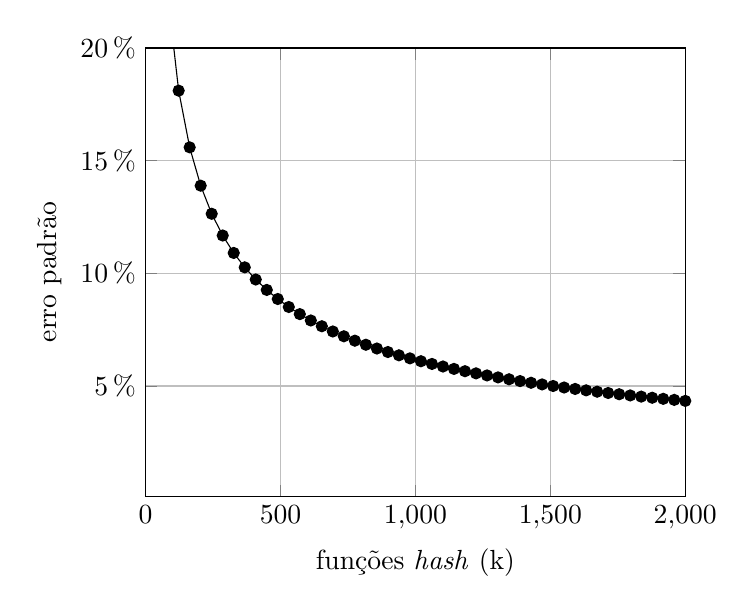
\begin{tikzpicture}[
        declare function = {
            p(\k,\c) = -(4 * sqrt(ln(2/\c)))/(sqrt(ln(2/\c))-sqrt(8*\k+ln(2/\c)));
        }
    ]
	\begin{axis}[
        grid=both,
        xlabel=funções \emph{hash} (k),
		ylabel=erro padrão,
		yticklabel=\pgfmathparse{100*\tick}\pgfmathprintnumber{\pgfmathresult}\,\%,
        ymin=0.001,
        ymax=0.20,
		xmin=0,
		xmax=2000]
	\addplot[mark=*,domain=0:2000,samples=50] {p(x, 0.317310508)};
	\end{axis}
\end{tikzpicture}}
\caption{Erro padrão por funções \emph{hash}}
\label{fig:min:prob}
\end{figure}

É razoável argumentar que para representar conjuntos arbitrários de cardinalidade $n$, seria necessário usar funções \emph{hash} de $O(\log n)$ bits. Entretanto, em \cite{b-bit-minwise-hashing}, Li e König argumentam que para qualquer esquema de \emph{hash} sensível a localidade (como \emph{MinHash}), guardar apenas um número constante dos bits menos significativos dos \emph{hashes} calculados não aumenta consideravelmente a variância dos estimadores para valores de similaridade próximos a 0,5.

\subsection{Variante com apenas uma função \emph{hash}}

Muitas vezes, o custo de computar várias funções \emph{hash} pode ser muito alto na prática, especialmente para conjuntos com centenas de milhões de elementos.

Uma variante possível do \emph{MinHash} é utilizar apenas uma função \emph{hash} e manter os $k$ menores resultados em ordem ascendente de $h(x)$ para cada conjunto como assinatura (Algoritmo~\ref{alg:min:hashcompute2}). Denota-se por $h_{(k)}(S)$ o conjunto com $k$ menores hashes do conjunto $S$ e $H_{\max}$ o valor máximo em $H$. 

\begin{algorithm}
\linespread{1}\selectfont
\caption{Computa a assinatura de um conjunto $S$}
\label{alg:min:hashcompute2}
\begin{algorithmic}[1]
\Function{Computar-Assinatura}{$S$}
    \State $H \gets \varnothing$
    \For{\text{each} $e \in S$}
        \State $H \gets H \cup h(e)$
        \If{$|H| > k$}
            \State $H \gets H - \{H_{\max}\}$
        \EndIf
    \EndFor
	\Return $H$
\EndFunction
\end{algorithmic}
\end{algorithm}

A similaridade entre os conjuntos será computada de uma forma diferente da variante com múltiplas funções \emph{hash}. Nesta, vale-se do princípio de que os $k$ menores elementos em $h_{(k)}(A) \cup h_{(k)}(B)$ são os mesmos que em $h_{(k)}(A \cup B)$. Assim, seja $Y = h_{(k)}(A \cup B) \cap h_{(k)}(A) \cap h_{(k)}(B)$.  $Y$ equivale aos membros de $h_{(k)}(A \cup B)$ que também estão em $ h_{(k)}(A \cap B)$. Pode-se, então, definir $|Y|/k$ como um estimador não-enviesado de $J(A, B)$ (Algoritmo~\ref{alg:min:hashcompare2}).

\begin{algorithm}
\linespread{1}\selectfont
\caption{Estima $J(A. B)$, sendo $H_1$ e $H_2$ as assinaturas, respectivamente, de $A$ e $B$}
\label{alg:min:hashcompare2}
\begin{algorithmic}[1]
\Function{Comparar-Assinaturas}{$H_1, H_2$}
    \State $H_x \gets k \text{ menores elementos de } H_1 \cup H_2 \ $
    \State $H_y \gets H_x \cap H_1 \cap H_2 $
	\Return $|H_y|/k$
\EndFunction
\end{algorithmic}
\end{algorithm}

Apesar da diferença prática, a ideia é similar à da variante com múltiplas funções \emph{hash}. Entretanto, nesta variante é preciso considerar que, em vez de obter apenas o primeiro elemento de cada permutação da matriz característica, obtém-se $k$ elementos. Mesmo assim, também é possível usar o limite de Chernoff para estimar o erro, pois o mesmo resultado para amostragem com substituição pode ser usado para amostragem sem substituição, como mostra Hoeffdin \cite{hoeffding1963probability,bardenet2015concentration}.

\subsection{Exemplo}\label{sec:minhash:example}

Com o objetivo de facilitar o entendimento da estrutura \emph{MinHash}, apresentamos aqui um exemplo prático de seu uso. Consideraremos aqui o cálculo da assinatura \emph{MinHash} de dois conjuntos $A$ e $B$, ambos contendo seis strings. Tal assinatura será computada através da variante com múltiplas funções \emph{hash}. São definidas $k=8$ funções \emph{hash} de 8 bits (por simplicidade). A Figura \ref{fig:minhash_example} mostra as tabelas que dão origem às assinaturas dos conjuntos.

\begin{figure}[!htbp]
  \centering
  \includegraphics[scale=0.6]{figures/minhash_example.pdf}
  \caption{Exemplos de construção de assinatura \emph{MinHash}}
  \label{fig:minhash_example}
\end{figure}

Cada linha de cada tabela corresponde a uma string, bem como os resultados da aplicação de cada função $h_1, \ldots, h_8$, no intervalo $[0; 255]$ (pois a função escolhida retorna valores de 8 bits). O rodapé da tabela mostra os valores mínimos para cada função. Esses valores compõem a assinatura de cada conjunto. A estimativa do índice de Jaccard se dá obtendo a proporção das posições nas assinaturas dos dois conjuntos que possuem o mesmo valor. No exemplo, metade dos valores são iguais entre as assinaturas (respectivos às funções $h_1$, $h_2$, $h_3$ e $h_6$). Considerando que no exemplo, de fato, $J(A, B) = 4/8 = 0,5$, podemos dizer que a estimativa foi precisa.

\subsection{Detecção de quase-duplicatas}\label{sec:min:duplicate}

A motivação inicial que levou à criação do algoritmo \emph{MinHash} era encontrar quase-duplicatas em uma coleção de 30 milhões de documentos indexados pelo motor de busca Alta Vista em 1997 \cite{broder1997resemblance}. Percebe-se que apenas considerando a técnica \emph{hashing}, a solução ainda é bastante impraticável, pois uma busca par-a-par no conjunto de dados requer $\binom{30,000,000}{2}$ -- ou aprox. 450 trilhões -- operações. Mesmo sendo capaz de executar cada comparação em 1 microsegundo, ainda levaria mais de uma década para processar a coleção inteira.

É importante notar, entretanto, que se o objetivo é encontrar grupos de similaridade, não é necessário computar o índice para todos os pares de conjuntos. É suficiente focar nos pares que possuem maior probabilidade de serem similares.

É possível utilizar a teoria \emph{hashes} sensíveis a localidade para diminuir a quantidade de pares a serem verificados. Uma técnica aplicável neste cenário é dividir as funções \emph{hash} em bandas e separar as assinaturas em baldes baseados no valor da assinatura em cada banda isoladamente. Assinaturas similares terão uma tendência maior de serem colocadas no mesmo balde (por terem valores idênticos de assinatura naquela banda), com uma probabilidade definida.

Para entender a técnica, considere múltiplos conjuntos e a matriz formada por suas assinaturas \emph{MinHash}, utilizando a variante com múltiplas funções \emph{hash}. Cada coluna representa um conjunto e cada linha representa uma função \emph{hash}. O objetivo é separar as linhas em bandas e, para cada banda, verificar os grupos de assinaturas formados como candidatos a duplicatas. 

Por exemplo, na Figura~\ref{fig:minhash_signaturematrix} ilustra-se uma matriz de assinatura representando 5 conjuntos e 8 funções \emph{hash}, divididas em 4 bandas com 2 linhas cada.

\begin{figure}[!htbp]
\centering
\begin{tabular}{ c | c || c | c | c | c | c }
 banda & hash & $S_1$ & $S_2$ & $S_3$ & $S_4$ & $S_5$ \\
\hline
  \multirow{2}{*}{1} & $h_1$ & 6   & 1   & 7   & 6  & 2   \\
                     & $h_2$ & 1   & 3   & 7   & 1  & 3   \\
\hline
  \multirow{2}{*}{2} & $h_3$ & 8   & 3   & 8   & 5  & 3   \\
                     & $h_4$ & 0   & 9   & 4   & 1  & 9   \\
\hline
  \multirow{2}{*}{3} & $h_5$ & 2   & 0   & 6   & 2  & 0   \\
                       & $h_6$ & 0   & 0   & 3   & 1  & 0   \\
\hline
  \multirow{2}{*}{4} & $h_7$ & 5   & 1   & 1   & 5  & 1   \\
                     & $h_8$ & 4   & 4   & 9   & 4  & 4   \\
\end{tabular}
\caption{Matriz de assinaturas}
\label{fig:minhash_signaturematrix}
\end{figure}

No exemplo, a banda 2 revela um potencial par de quase-duplicatas, pois $S_2$ e $S_5$ possuem o mesmo valor para suas assinaturas naquela banda.

Considerando que deseja-se encontrar pares com similaridade acima de um certo limite, esta técnica está sujeita tanto a falsos positivos quantos falsos negativos. A probabilidade de um par de conjuntos $A$ e $B$, com $J(A, B) = s$, ser marcado como potencial duplicata, numa matriz com $b$ bandas com $r$ linhas por banda é exatamente a probabilidade dos dois conjuntos concordarem em todas as linhas de pelo menos uma banda, que é de $1 - (1 - s^r)^b$  \cite{rajaraman2012mining}.

Baseado nesta probabilidade, a Figura~\ref{fig:min:lshprob} mostra, em função da similaridade, a probabilidade de um par de documentos ser marcado como duplicado em uma matriz com 64 funções \emph{hash} e algumas escolhas de $b$ diferentes.

\begin{figure}[!htbp]
\centering
\scalebox{0.80}{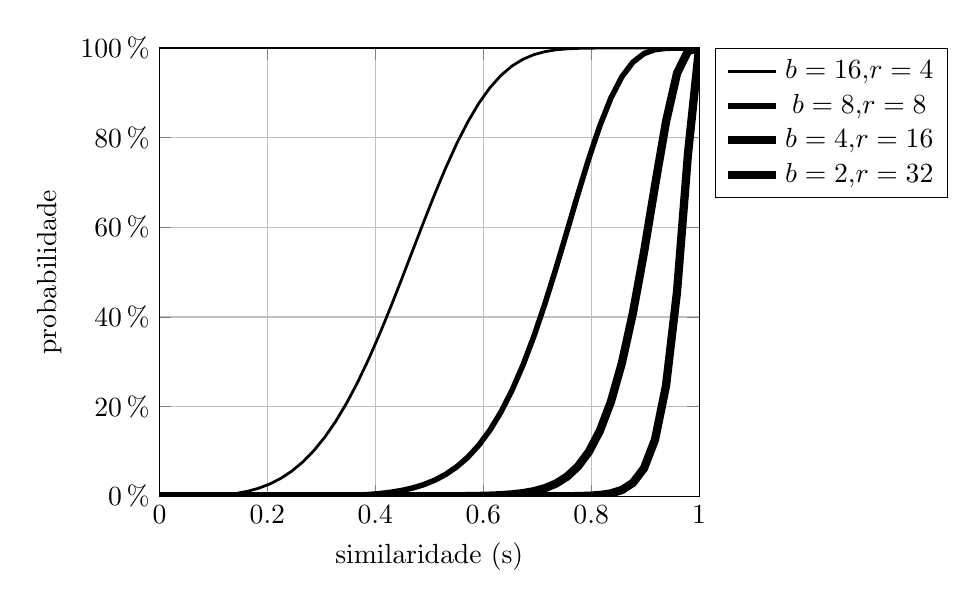
\begin{tikzpicture}[
        declare function = {
            p(\s,\b,\r) = 1 - (1 - \s^\r)^\b;
        }
    ]
	\begin{axis}[
        grid=both,
        xlabel=similaridade (s),
		ylabel=probabilidade,
		yticklabel=\pgfmathparse{100*\tick}\pgfmathprintnumber{\pgfmathresult}\,\%,
		ymin=0, ymax=1,
		xmin=0, xmax=1, 
		legend columns=1, 
	    legend style={legend pos=outer north east,}]
	\addplot[line width=1pt,domain=0:1,samples=50] {p(x, 16, 4)};
	\addplot[line width=2pt,domain=0:1,samples=50] {p(x, 8, 8)};
	\addplot[line width=3pt,domain=0:1,samples=50] {p(x, 4, 16)};
	\addplot[line width=3pt,domain=0:1,samples=50] {p(x, 2, 32)};
	\legend{$b=16 \text{, } r=4$, $b=8 \text{, } r=8$, $b=4 \text{, } r=16$, $b=2 \text{, } r=32$}
	\end{axis}
\end{tikzpicture}}
\caption{Probabilidade de ser escolhido como duplicata}
\label{fig:min:lshprob}
\end{figure}

Independente dos valores de $b$ e $r$ escolhidos, o gráfico sempre terá esta forma de "S". Entretanto, estes parâmetros definem com qual probabilidade um par de certa similaridade $s$ é considerado duplicado. Ainda assim, valores abaixo da similaridade definida podem ser considerados duplicados (falsos positivos) e valores acima podem ser ignorados (falsos negativos). 

A partir de $b$ e $r$ e uma probabilidade $p$ é possível derivar a partir de qual valor de similaridade se possui aquela probabilidade de ser escolhido, por inversão da função que fornece esta probabilidade:
\[
s = \left(1 - (1-p)^{1/b}\right)^{1/r}
\]

Por exemplo, $b=32$, $r=16$, temos 0,5\% de chance de encontrar um par de conjuntos com similaridade acima de $0,5683$, e 95\% de chance de encontrar pares com similaridade acima de $0,8891$. Ao manipular estes valores é possível dimensionar facilmente a tolerância a falsos positivos ou falsos negativos no algoritmo.

\subsection{\emph{SimHash}}

A partir do trabalho de Indyk e Motwani \cite{indyk1998approximate,gionis1999similarity}, começou-se a formalizar as bases teóricas das técnicas \emph{hashing} sensível a localidade. De fato, \emph{MinHash} é apenas um tipo destes hashes. Muitos outros tipos foram estudados desde então. Uma dos mais bem sucedidos é o \emph{SimHash} \cite{charikar2002similarity}. Este algoritmo ganhou notoriedade nos últimos anos por compor um dos fatores usados pelo Google para priorizar a indexação de páginas na Internet \cite{manku2007detecting}.

Um hash sensível a localidade é definido por uma família de funções \emph{hash} $\mathcal{F}$, tal que para dois elementos $x, y \in U$, e uma certa função de similaridade $sim: U \times U \to [0, 1]$, vale
\[
    \Pr_{h \in \mathcal{F}}[h(x) = h(y)] = sim(x, y)
\]

Em especial, para o \emph{MinHash}, o objetivo é estimar a similaridade entre conjuntos com um número grande de elementos, aproximando o índice de Jaccard, i.e. $sim(x, y) = J(x, y)$. Outras medidas podem ser utilizadas. 

No caso das assinaturas de Charikar -- ou \emph{SimHash} -- o objetivo é estimar a similaridade entre vetores em espaços de alta dimensão. Neste caso utiliza-se uma família de funções \emph{hash} baseadas no produto escalar entre vetores. No algoritmo, para comparar a similaridade em vetores em $\mathds{R}^d$, escolhe-se um vetor $\vec{r}$, de $d$ dimensões, onde cada coordenada é um valor escolhido aleatoriamente em uma distribuição gaussiana. Define-se a função como \[
    h_{\vec{r}}(\vec{u}) = \begin{cases} 
        1 & \text{se } \vec{r} \cdot \vec{u} \geq 0 \\
        0 & \text{se } \vec{r} \cdot \vec{u} < 0 \\
    \end{cases}
\]

Goemans e Williamson \cite{goemans1995improved} mostram que esta função pode ser utilizada como um hash sensível a localidade, tal que, para vetores $\vec{u}$ e $\vec{v}$,
\[
    \Pr[h_{\vec{r}}(\vec{u}) = h_{\vec{r}}(\vec{v})] = 1 - \frac{\theta(\vec{u}, \vec{v})}{\pi}\text{, }
\] 
onde $\theta(\vec{u}, \vec{v})$ é o menor ângulo formado por $\vec{u}$ e $\vec{v}$.

É possível utilizar esta família de funções para estimar a similaridade entre conjuntos. Cada elemento da união dos dois conjuntos seria associado a uma dimensão e cada conjunto representado como um vetor, tendo valor 1 nas dimensões respectivas aos elementos que contém. Por exemplo, sejam dois conjuntos $A$ e $B$:
\[
    A = \{a, d, e\} \text{ e } \\
    B = \{b, c, d, e\}
\]
uma possível definição dos vetores relativos a $A$ e $B$ seria:
\[
    v_A = (1, 0, 0, 1, 1) \text{ e } 
    v_B = (0, 1, 1, 1, 1)
\]

Como o menor ângulo formado por estes dois vetores é 1,15026 rad, então a similaridade entre os dois, segundo esta métrica, é igual a aproximadamente 0.695913. Para conjuntos, esta função \emph{hash} (tal associação de vetores a elementos) representa a seguinte métrica de similaridade:

\[
    \Pr[h_{\vec{r}}(\vec{u}_A) = h_{\vec{r}}(\vec{u}_B)] = 1 - \frac{\arccos \left( \frac{|A \cap B|}{\sqrt{|A| \cdot |B|}}\right)}{\pi}\text{.}
\]

Na prática, o algoritmo consiste em computar $k$ bits, armazenados em um vector $V[1..k]$, onde o elemento $V[i]$ assume valor $0$ se, usando-se a $i$-ésima função \emph{hash}, houver menos elementos no conjunto com valor \emph{hash} negativo do que não-negativo, ou assume valor $1$ caso contrário (Algoritmo~\ref{alg:min:simhashcompute}).

\begin{algorithm}
\linespread{1}\selectfont
\caption{Computa a assinatura \emph{SimHash} de um conjunto $S$}
\label{alg:min:simhashcompute}
\begin{algorithmic}[1]
\Function{Computar-Assinatura}{$S$}
    \For{$i \gets 1 \textrm{ to } k$}
        \State $v \gets 0$
        \For{\text{each} $e \in S$}
            \If{$h_i(e) \geq 0$}
                \State $v \gets v + 1$
            \Else
                \State $v \gets v - 1$
            \EndIf
	    \EndFor
        \State $H[i] \gets (v \geq 0)$
	\EndFor
	\Return $H$
\EndFunction
\end{algorithmic}
\end{algorithm}

A comparação entre duas assinaturas consiste em determinar a proporção de bits iguais nas assinaturas (Algoritmo~\ref{alg:min:simhashcompare}).

\begin{algorithm}
\linespread{1}\selectfont
\caption{Compara assinaturas \emph{SimHash} de conjuntos}
\label{alg:min:simhashcompare}
\begin{algorithmic}[1]
\Function{Comparar-Assinaturas}{$H_1, H_2$}
    \State $y \gets 0$
    \For{$i \gets 1 \textrm{ to } k$}
        \If{$H_1[i] = H_2[i]$}
            \State $y \gets y + 1$
        \EndIf
	\EndFor
	\Return $y/k$
\EndFunction
\end{algorithmic}
\end{algorithm}

Henzinger \cite{henzinger2006finding} argumenta que \emph{SimHash} tem um desempenho melhor ao estimar quase-duplicatas em documentos na Internet, se comparado ao \emph{MinHash}. Em especial, \emph{SimHash} requer menos espaço para atingir mesma precisão que \emph{MinHash}. Por outro lado, Shrivastava e Li \cite{shrivastava2014defense} afirmam que \emph{MinHash} é mais adequado que \emph{SimHash} para coleções de documentos com muitas similaridades.

Manku et al. \cite{manku2007detecting} descrevem a aplicabilidade desta técnica para detecção de quase-duplicatas usando assinaturas de 64 bits num banco de dados de 8 bilhões de páginas. Também sugerem um algoritmo otimizado para encontrar todas as assinaturas que diferem de uma assinatura específica em no máximo $k$ bits, onde $k$ é um inteiro pequeno.

\subsection{Aplicações}

O algoritmo \emph{MinHash} e outros mecanismos \emph{hash} sensíveis a localidade, têm enorme aplicação prática, especialmente como forma de oferecer uma função de similaridade e algoritmos de clusterização para os mais variados fins. Nesta seção listaremos alguns exemplos de aplicações comuns nesta área.

\begin{description}

\item[Sites de busca:]

Em seu trabalho seminal sobre \emph{MinHash}, Broder \cite{broder1997resemblance} já citava uma aplicação prática na indexação de páginas web pelo motor do Alta Vista, numa análise investigativa a fim de determinar quase-duplicatas em um índice de 30 milhões de documentos.

Manku et al. \cite{manku2007detecting} descrevem como usam, no Google, outra variante \emph{hash} sensível a localidade chamada \emph{SimHash}, baseada em distância entre vetores. No artigo, os autores introduzem uma técnica para determinar, a partir de coleção de 8 bilhões de páginas com assinaturas \emph{SimHash} de 64 bits pré-calculadas, se uma nova página encontrada pelo indexador possui uma duplicata já indexada.

\item[Bancos de dados de imagens:]

Embora hashing sensível a localidade seja mais comumente usado para comparação de documentos textuais, também é possível adaptá-lo para comparar a semelhança entre imagens. Neste caso, várias caracteristicas da imagem podem ser usadas como meio de comparação, desde histogramas de cores, parâmetros de iluminação, até os pixels individuais.

Ioffe \cite{ioffe2010improved} cita um caso de uso para uma variante do algoritmo \emph{MinHash}, modificada para permitir conjuntos ponderados, de modo a aproximar a distância $\ell_1$ entre vetores. No artigo, o objetivo principal é apresentar o uso da técnica, no Google, para busca aproximada por imagens num banco de dados. As imagens são representadas por vetores de features, como histogramas de cores e metadados. 

Lee et al. \cite{lee2010partition} também descrevem um método para busca parcial de imagens usando \emph{MinHash}. Neste caso, o objetivo é agrupar imagens que provavelmente contém um mesmo objeto, mesmo que as imagens não sejam inteiramente compostas por ele.

Numa aplicação mais clássica, Wang et al. \cite{wang2013duplicate} expõem os resultados alcançados pela divisão Microsoft Research em uma busca por duplicatas em uma coleção de mais de 2 bilhões de imagens da Internet. Utilizando uma variante em dois passos do \emph{MinHash}, eles foram capazes de encontrar mais de 500 milhões de imagens duplicadas em 13 horas de processamento em um cluster de 2.000 núcleos.

\item[Sistemas de recomendação:]

A capacidade de verificar a semelhança entre conjuntos ou vetores abre portas para aplicação de \emph{MinHash} em algoritmos de clusterização baseados em similaridade.

O serviço de notícias Google News utiliza \emph{MinHash} para seu mecanismo de recomendação de artigos para os usuários \cite{das2007google}. A recomendação é calculada em tempo real com latência abaixo de um segundo. Para tanto, os autores descrevem como utilizam aprendizado de máquina, aplicando \emph{MinHash} como função de similaridade. Todo o processamento é realizado no modelo MapReduce, para permitir a criação de um mecanismo de recomendação de notícias com alta escalabilidade.

Além disso, Rodrigues \cite{rodrigues2013recomendaccao} sugere a utilização de \emph{MinHash} para clusterização de espectadores em serviços de TV, baseados nas opções pregressas.

\item[Similaridade em Redes Sociais:]

A detecção de comunidades orgânicas em redes sociais é um problema cada vez mais comum atualmente. O problema pode ser modelado como um caso especial de sistema de recomendação, onde o objetivo é clusterizar nós comuns num grafo por um conjunto de características. 

Macropol e Singh \cite{macropol2010scalable} introduzem em 2010 o algoritmo \emph{Top Graph Clusters} (\emph{TopGC}), utilizando hashes sensíveis a localidade -- especialmente \emph{MinHash} -- para detecção, em tempo linear, de subgrafos altamente conectados. O algoritmo propõe utilizar, como métrica de afinidade entre os nós, a semelhança entre suas vizinhanças.

Teixeira et al. \cite{teixeira2012min} descrevem como utilizar \emph{MinHash} como função de similaridade, com o objetivo de computar a semelhança entre grafos utilizando poucos recursos.


\end{description}

\subsection{Resultados experimentais}\label{sec:min:experiments}

Para melhor observar as previsões teóricas sobre o algoritmo \emph{MinHash}, conduzimos uma série de experimentos para verificar empiricamente as probabilidades descritas na teoria. Testamos tanto a variante com múltiplas funções \emph{hash} quanto com apenas uma função. Testamos também a técnica de clusterização de pares duplicados descrita na Seção~\ref{sec:min:duplicate}.

Para todos os testes, foi utilizado um conjunto de dados misto, composto por todas as obras de Shakespeare (42 obras, 964410 palavras, 23704 distintas). Para cada obra, consta no conjunto de dados o conjunto de palavras distintas da obra, bem como uma cópia deste conjunto com uma certa porcentagem aleatória de palavras substituídas por strings aleatórias (84 conjuntos de palavras foram utilizados no total).

Em todos os casos, a família de funções \emph{hash} utilizada foi MurmurHash 3 \cite{appleby2012murmur}, de 32 bits. Várias funções foram geradas, usando sementes diferentes.

A métrica de similaridade utilizada no teste foi o índice de Jaccard entre os conjuntos simples de palavras de cada texto. Este índice foi calculado de forma determinística para os $\binom{42 \times 2}{2} = 3486$ pares de documentos. A distribuição de similaridades entre os pares pode ser vista no histograma da Figura~\ref{fig:minhash_dist}.

\begin{figure}[!htbp]
\centering
\scalebox{0.80}{\begin{tikzpicture}
	\begin{semilogyaxis}[
	    ybar,
	    xmin=0, xmax=1,
        ylabel={quantidade},
        xlabel={similaridade},
    ]

    \addplot +[
        fill=gray!25,
        draw=gray!100,
        hist={
            bins=10,
            data min=0,
            data max=1
        }   
    ] table [y index=0] {files/minhash_dist.txt};

	\end{semilogyaxis}
\end{tikzpicture}}
\caption{Distribuição de similaridades entre pares de documentos}
\label{fig:minhash_dist}
\end{figure}


Para os dois testes, variou-se $k$ (o número de funções \emph{hash}) entre 25 e 1000. Mediu-se então, para cada par, o quanto o estimador da similaridade desviava do valor real (calculado deterministicamente). Para estes valores foram computados a média, e o desvio padrão. A Figura \ref{fig:min:result} mostra os resultados obtidos para as variantes de múltiplas funções e apenas uma função \emph{hash}, respectivamente. Na figura é possível comparar com o intervalo esperado pela teoria apresentada, com 95\% de certeza.

\begin{figure}[!htbp]
\centering
\scalebox{0.80}{\begin{tikzpicture}[
        declare function = {
            p(\k,\c) = -(4 * sqrt(ln(2/\c)))/(sqrt(ln(2/\c))-sqrt(8*\k+ln(2/\c)));
        }
    ]
	\begin{axis}[
	    title=Múltiplas funções \emph{hash},
	    scaled ticks=false, 
        grid=both,
        ylabel={erro},
        xlabel=tamanho da assinatura ($k$),
		yticklabel=\pgfmathparse{100*\tick}\pgfmathprintnumber{\pgfmathresult}\,\%,
		ymin=0,ymax=0.3,ystep=0.01,
		xmin=0, xmax=1000, 
		legend columns=1, 
	    legend style={legend pos=outer north east,}
    ]

    \addplot[line width=15pt,domain=0:1,samples=30,color={rgb:black,1;white,1},opacity=0.4]{2};

    \addplot[name path=line3, line width=0pt,domain=1:1000,samples=40,opacity=0.0,forget plot]{p(x, 0.05)};
    \addplot[name path=line4, line width=15pt,domain=1:1000,samples=30,opacity=0.0, forget plot]{0};

	\addplot[fill={rgb:black,1;white,1},fill opacity=0.40,forget plot] fill between[ of = line3 and line4];

	\addplot[line width=1pt, mark=*,black,smooth, mark options={scale=0.75}] table[x=k,y=mean] {files/minhash_shakespeare.txt};
	\addplot[dashed, line width=1pt, mark=none,black,smooth, mark options={scale=0.75}] table[x=k,y=stdev] {files/minhash_shakespeare.txt};
	%\addplot[dotted, line width=1pt, mark=none,black,smooth] table[x=k,y=max] {files/minhash_shakespeare.txt};
	%\legend{esperado,shakespeare, $\pm 1 \sigma$, min/max };


	\end{axis}
\end{tikzpicture} \begin{tikzpicture}[
        declare function = {
            p(\k,\c) = -(4 * sqrt(ln(2/\c)))/(sqrt(ln(2/\c))-sqrt(8*\k+ln(2/\c)));
        }
    ]
	\begin{axis}[
	    title=Única função \emph{hash},
	    scaled ticks=false, 
        grid=both,
        xlabel=tamanho da assinatura ($k$),
		yticklabel={\ },
		ymin=0,ymax=0.3,ystep=0.01,
		xmin=0, xmax=1000, 
		legend columns=1, 
	    %legend style={legend pos=outer north east,}
    ]

    \addplot[line width=15pt,domain=0:1,samples=30,color={rgb:black,1;white,1},opacity=0.4]{2};

    \addplot[name path=line3, line width=0pt,domain=1:1000,samples=40,opacity=0.0,forget plot]{p(\x, 0.05)};
    \addplot[name path=line4, line width=15pt,domain=1:1000,samples=30,opacity=0.0, forget plot]{0};
	\addplot[fill={rgb:black,1;white,1},fill opacity=0.40,forget plot] fill between[ of = line3 and line4];

	\addplot[line width=1pt, mark=*,black,smooth, mark options={scale=0.75}] table[x=k,y=mean] {files/minhash_shakespeare2.txt};
	\addplot[dashed, line width=1pt, mark=none,black,smooth, mark options={scale=0.75}] table[x=k,y=stdev] {files/minhash_shakespeare2.txt};
	%\addplot[dotted, line width=1pt, mark=none,black,smooth] table[x=k,y=max] {files/minhash_shakespeare2.txt};
	\legend{esperado, média, $+1\sigma$, máximo };

	\end{axis}
\end{tikzpicture}}
\caption{Erro observado por funções \emph{hash}}
\label{fig:min:result}
\end{figure}

Também foi testada a técnica de detecção de duplicatas descrita na Seção~\ref{sec:min:duplicate}. 

Inicialmente calculou-se, para cada documento, assinaturas \emph{MinHash} com 512 funções \emph{hash}. Utilizou-se então a técnica de detecção de duplicatas utilizando todas as possíveis combinações de número de bandas ($b$) e linhas por banda ($r$). 

\begin{figure}[!htbp]
\centering
\scalebox{0.80}{\begin{tikzpicture}[
        declare function = {
            p(\b,\r,\p) = (1 - (1-\p)^(1/\b))^(1/\r);
        }
    ]
	\begin{axis}[
	    xmode=log,
	    log basis x=2,
	    scaled ticks=false, 
        grid=both,
        xlabel=número de bandas ($b$),
		ylabel=similaridade ($s$),
		ymin=0,ymax=1,
		xmin=8,xmax=512, 
		legend columns=1, 
	    legend style={legend pos=outer north east,},
	    legend cell align=left
    ]

    \addplot[line width=15pt,domain=8:9,samples=2,color={rgb:black,1;white,1},opacity=0.4]{2};
    \addplot[line width=15pt,domain=8:9,samples=2,color={rgb:black,1;white,1},opacity=0.7]{2};


    \addplot[name path=line3, line width=0pt,domain=8:512,samples=40,opacity=0.0,forget plot] table[x=b,y=max] {files/minhash_calculated.txt};
    \addplot[name path=line4, line width=0pt,domain=8:512,samples=40,opacity=0.0,forget plot] table[x=b,y=min] {files/minhash_calculated.txt};
    \addplot[name path=line5, line width=0pt,domain=8:512,samples=40,opacity=0.0,forget plot]{1};
	\addplot[fill={rgb:black,1;white,1},fill opacity=0.40,forget plot] fill between[ of = line3 and line4];
	\addplot[fill={rgb:black,1;white,1},fill opacity=0.70,forget plot] fill between[ of = line5 and line3];

	\addplot[only marks, mark=*,opacity=1,black,mark options={scale=0.75}] table[x=b,y=v] {files/minhash_detect.txt};
    
    \legend{{$0,5\%<P<99,5\%$},{$P\geq99,5\%$}, pares encontrados };


	\end{axis}
\end{tikzpicture}}
\caption{Pares detectados para cada configuração de bandas.}
\label{fig:min:detect}
\end{figure}

As similaridades dos pares encontrados com cada configuração, bem como a comparação com o valor predito pela teoria podem ser vistos na Figura~\ref{fig:min:detect}. Configurações que resultaram em nenhum par encontrado são omitidas por brevidade.

É importante notar no resultado não só valores abaixo da probabilidade de corte (falsos positivos), como muitos valores de similaridade altos omitidos numa certa configuração de bandas, mas que aparecem na próxima (falsos negativos).
\input{3x4_hyperloglog}



\section{Considerações sobre as estruturas}

Neste capítulo, apresentamos quatro estruturas de dados importantes para a representação probabilística de conjuntos. Cada uma delas permite certas operações sobre os conjuntos que representam. Nesta seção, destacaremos as similaridades e diferenças entre essas estruturas. A Figura~\ref{fig:probds_table2} revisa a tabela apresentada no início do capítulo, que resume as estruturas apresentadas nas seções anteriores, incluindo os parâmetros e o cálculo do limite superior do erro descritos ao longo do capítulo.

\begin{figure}[!htbp]
\centering
\scalebox{0.78}{\begin{tabular}{ | c | c | c | c | N}
\hline
    \textbf{Estrutura} & \textbf{Parâmetros} & \textbf{Consulta} & \textbf{Erro} &\\[10pt]
\hline
\hline
    \multirow{2}{*}{Filtro de Bloom} &     
    \multirow{2}{*}{\shortstack{$m$ bits \\ $k$ funções \emph{hash}}} & 
    Pertinência & 
    $\Pr[\textsc{FalsoPositivo}] \approx 0,6185^{m/n}$  &\\[17pt]
\cline{3-4}
    & & Cardinalidade & 
    $\sigma_{\hat{n}} = \frac{\sqrt{m(e^{n/m} - (n/m) - 1)}}{n}$  &\\[17pt]
\hline
\hline
    \multirow{3}{*}{Count-Min sketch} &      
    \multirow{3}{*}{\shortstack{$m = \lceil e/\epsilon \rceil$ \\ $k = \lceil \ln(1/\delta) \rceil$}} & 
    Frequência & 
    $\Pr\left[ \widehat{A[i]} > A[i] + \epsilon \lVert A \rVert_1 \right] \leq \delta$  &\\[17pt]
\cline{3-4}
    & & Produto escalar & 
    $\Pr\left[ \widehat{A \cdot B} > A \cdot B + \epsilon \lVert A \rVert_1 \lVert B \rVert_1 \right] \leq \delta$  &\\[17pt]
\cline{3-4}
    & & Somatório de intervalos & 
    $\Pr\left[ \widehat{Q(a, b)} > Q(a, b) + 2 \epsilon \log_2 n \lVert A \rVert_1 \right] \leq \delta$ &\\[17pt]
\hline
\hline
  MinHash & 
  $k \geq \frac{2+\theta}{\theta^2} \times \ln(2/\delta)$ & 
  Similaridade & 
  $ \Pr\left[ \left| \frac{\hat{J(A, B)}}{J(A,B)} -1 \right| > \theta \right] \leq \delta $ &\\[17pt]
\hline
\hline
  HyperLogLog & 
  $m \times \lceil \log \log n \rceil$ bits & 
  Cardinalidade & 
  $\sigma_{\hat{n}} \approx 1,03896/\sqrt{m}$ &\\[17pt]
\hline
\end{tabular}}
\caption{Sumário de estruturas abordadas neste capítulo}
\label{fig:probds_table2}
\end{figure}

\subsection{filtro de Bloom e \emph{Count-Min sketch}}

É possível perceber uma certa semelhança na construção das estruturas filtro de Bloom e \emph{Count-Min sketch}. Além disso, são as únicas estruturas dentre as quatro que possuem complexidade de espaço linear. De fato, \emph{Count-Min sketch} é descrita na literatura como uma variante de um filtro de Bloom, conhecida como \emph{Spectral Bloom filter} \cite{cohen2003spectral}. É possível, entretanto, prever a probabilidade de erro (falsos positivos) no filtro de Bloom com certa segurança. No caso de \emph{Count-Min sketch} é preciso recorrer à desigualdade de Markov para definir um limite superior no erro da estimativa da frequência de elementos específicos. Por este motivo, seu erro teórico é superestimado. Por outro lado, \emph{Count-Min} permite outras operações quando usada para representar vetores: é possível estimar também o produto escalar usando a mesma estrutura e o somatório de intervalos de elementos no vetor com uma simples adaptação na representação.

\subsection{\emph{MinHash} e \emph{HyperLogLog}}

\emph{MinHash} e \emph{HyperLogLog} são menos ``versáteis'' se comparadas as outras estruturas, porém ambas possuem complexidade de espaço sublinear. São especializadas em estimar um parâmetro apenas: similaridade de Jaccard entre conjuntos, no caso do \emph{MinHash} e cardinalidade de elementos distintos em multiconjuntos, no caso do \emph{HyperLogLog}. Ambas as estruturas baseiam-se na definição de um estimador para a métrica que representam e na composição desses estimadores para redução da variância. No caso de \emph{MinHash}, o estimador é definido pelo menor resultado de uma função \emph{hash} aplicada a cada elemento do conjunto; a probabilidade de dois conjuntos terem o mesmo menor elemento é igual à similaridade de Jaccard entre os dois. No caso do \emph{HyperLogLog}, o estimador é definido pelo maior prefixo $0^{p-1}1$ visto na representação binária do resultado de uma função \emph{hash} aplicada a cada elemento do multiconjunto; a estimativa da cardinalidade de elementos distintos é dada por $2^p$.

Há sinergia entre \emph{MinHash} e \emph{HyperLogLog} também para estimar a cardinalidade da interseção de conjuntos. Dado que, para dois conjuntos $A$ e $B$, \emph{MinHash} permite estimar $\frac{|A \cap B|}{|A \cup B|}$ e \emph{HyperLogLog} permite estimar $|A \cup B|$, combinando as duas estruturas é possível estimar a cardinalidade $|A \cap B|$ com erro relativo apenas ao tamanho da interseção dos conjuntos.